% RENUMBERED 2026-11-16 (user: "rename the files also"): methodology files follow the reading order.
%   Old -> new: 05 features -> 03 (05a/05b/05c -> 03a/03b/03c), 06 feature validity -> 04,
%   03 statistical model (before that 03_prediction_model) -> 05, 04 model size -> 06; 07 unchanged.
%   File names in the comments below were updated; bare numbers in comments dated before this entry
%   ("Methods 03", "05a header", "05d") are the OLD numbers.
% Technical Background, section 1: the cloglog GLMM, its hazard ratios, the likelihood ratio test of a
% set of covariates and the cluster risk. General method only, present tense; no cohort numbers,
% settings or software (Methodology 03).
% The dated edit log up to 2026-11-16 was moved out of this file to
%   research_notes/Mixed model study note/01_mixed_model_changelog.md
% The elementary explanations cut from this section are kept, with worked examples, in the study note
%   research_notes/Mixed model study note/mixed_model_explainer.tex (not part of the thesis).
% Copy before the review fixes of 2026-11-16: scratchpad 01_mixed_model_before_review_fixes.tex.
%
% SOURCES BY LOCATION
% dobson2002glm (PDF in the repository root; re-read 2026-11-16): 3.4 (GLM; "monotone, differentiable
%   function called the link function"; "a set of independent random variables"), 7.2 (a linear model
%   for a probability can give fitted values below 0 or above 1), 7.3 (name of the cloglog link, from a
%   dose-response model, not from hazards), 10.2 and Eq. 10.4 (hazard, cumulative hazard,
%   S = exp[-H]), 10.2.2 Eq. 10.8 (proportional hazards) and Eq. 10.7 (hazard ratio e^{beta_k}
%   "provided that sum_{i != k} x_i beta_i is constant"), 9.2 Eq. 9.3 (offset; stated for Poisson
%   regression with a log link, not for a cloglog model), 11.1 (correlated outcomes; "models that
%   include correlation are needed in order to make valid statistical inferences"), 11.5 (random
%   effect, "fixed effect", "a mixed model with both fixed and random effects"; g(mu) = X beta + Z u),
%   5.7 and 11.7 (likelihood ratio statistic for nested models; "For multilevel data, nested models can
%   be compared using likelihood ratio statistics").
% austin2017mhr (PMC5299617, Section 2.2 and Discussion, re-read 2026-11-16 through a web fetch): "the
%   term e^{alpha_j} is referred to as a frailty term", "The frailty terms have a multiplicative effect
%   on the hazard function"; the MHR is "the median relative change in the hazard ... when comparing
%   identical subjects" from two randomly selected clusters, ordered by risk; "for 50% of possible
%   pair-wise comparisons". SETTING: a Cox model with log-normal frailty, not a cloglog GLMM.
%
% CHECK: prentice1978grouped pp. 58-59, Eqs. 2-5 (the cloglog risk from grouped proportional hazards)
%   was read by an earlier session from pasted text and has not been opened since. No PDF in the
%   repository. The \cite on eq:tech-cloglog rests on it; put the PDF in papers/ and verify.
% CITATION WANTED: a multilevel text that states the general rule for standard errors under clustering
%   (too small for covariates that differ between clusters, can be too large for covariates that differ
%   within). Dobson shows it only as one example (11.6, Table 11.7), so the rule was removed from the
%   text on 2026-11-16 and replaced by what 11.1 states (inference is not valid).
% CHECK: Methodology 03 must name the confidence interval the final script reports (Wald or profile).
% CAREFUL: Dobson's q in 5.7 is the number of parameters of the simpler model (df = p - q); here q is
%   the number of added covariates.
% CAREFUL: Dobson never writes that the cloglog link "assumes" proportional hazards. The text says the
%   link arises from the hazard description and that the hazard-ratio reading holds under proportional
%   hazards.
%
% UNCITED REASONING (follows from the equations): "the two are connected by ... whose inverse maps";
%   Lambda_i = exp(eta_i) with the baseline in the intercept (Dobson 10.2.2, line before Eq. 10.9, with
%   log H0 as the intercept); "referred to as adjusted" (the word is not Dobson's); gamma log E_i with
%   gamma estimated; "a cluster with a frailty above 1 is more prone"; "an MHR of 2 means that in half
%   of such pairs" (definition of a median); the conditional reading of exp(beta_k) for covariates that
%   vary within or between clusters (follows from eq:tech-glmm; austin2017mhr does not discuss it);
%   estimation by maximum likelihood with the likelihood averaged over b_i (sources are in
%   app:glmm-fitting); the dilution of one unit in H_i; "The link follows from an event that can occur
%   at any time within the observation window but is observed only at its end" (2026-11-16; shown by
%   the next sentences via Dobson Eq. 10.4; replaced "commonly used when the event is described through
%   its hazard", which Dobson does not state). CHECK: suresh2022discrete (BMC Med Res Methodol 22:207,
%   open access) calls the cloglog model the grouped proportional hazards model for continuous time
%   divided into intervals; seen only as a web summary, not cited. Put the PDF in papers/ before use.
% 2026-11-16 (user: "can the derivation be written out" -> "yes put it in"): "Summed over the window ..."
%   replaced by eq:tech-cumhaz (Lambda_i as the integral of h_i(t) over [0, tau], 1 - p_i = exp(-Lambda_i)),
%   Dobson 10.2 Eq. 10.4 (S(y) = exp[-H(y)], H(y) = integral of h). New notation: h_i(t), t, tau
%   (tau, not T, which is the average curvature in Methods 05a).
% 2026-11-16 (user: "should eta = log Lambda go into the thesis" -> "yes put it in"): the sentences "The linear
%   predictor is then the logarithm ..." and "With Lambda_i = exp(eta_i), the risk becomes" replaced by
%   eq:tech-logcumhaz (log Lambda_i = log Lambda_0 + sum beta_k x_ik = eta_i; beta_0 = log Lambda_0). Source:
%   Dobson 10.2.2, unnumbered display before Eq. 10.9 (log H1 = log H0 + sum x_i beta_i, from
%   H1 = H0 e^{x'beta}); beta_0 = log Lambda_0 is our step (Dobson keeps H0 as a baseline, no intercept).
%   eq:tech-cloglog now follows by substitution from eq:tech-cumhaz and eq:tech-logcumhaz, so the
%   prentice1978grouped cite was removed from this section. Its CHECK above still applies to Appendix B and
%   Methods 03, which cite it.
% 2026-11-16 (user: "rewrite ... to have the necessary equations and for them to come in the optimal order"):
%   ADDED eq:tech-ph (h_i(t) = h_0(t) exp(sum beta_k x_ik), Dobson 10.2.2 Eq. 10.8; "baseline hazard" is Dobson's
%   term) between eq:tech-cumhaz and eq:tech-logcumhaz, so the chain hazard -> cumulative hazard -> proportional
%   hazards -> log cumulative hazard -> risk and link is complete. eq:tech-cloglog now also gives the link
%   g(p) = log{-log(1 - p)} (Dobson 7.3: "log[-log(1 - pi)] ... is called the complementary log log function").
%   The hazard-ratio sentence now starts from eq:tech-ph (Eq. 10.7 follows from 10.8) and says "at every time in
%   the window"; the exposure sentence points to eq:tech-logcumhaz. All labels kept. Appendix B
%   (eq:app-link-ph, eq:app-link-cloglog and the name sentence) now repeats this derivation; trim it to the worked
%   example and the logit comparison when the appendix is next revised.
% 2026-11-16 (user: "yes move the citation"): Dobson 7.3 moved from "solving for eta_i gives the link itself" to the
%   naming sentence. 7.3 gives the form log[-log(1 - pi)] and the name, but reaches it from an extreme-value
%   tolerance distribution, not from a hazard; the derivation here combines 10.2 (Eq. 10.4) and 10.2.2 and is
%   uncited as a step.
% 2026-11-16 (user: "write this more easily understandable"): "Since the other covariates are held fixed, the
%   hazard ratio is adjusted for them. A hazard ratio refers to one unit of its covariate and is read together
%   with that unit." -> units that agree on all other covariates; worked example 1.1 per year = 1.1^10 = 2.59,
%   written 2.6, per ten years (made-up number, own computation).
%
% 2026-11-16 (user: "make the changes to the issues just identified"; review of the section against
%   Aida's Chapter 3). CHANGED:
%   - "which we here call the risk" -> "referred to as the risk" (no first person).
%   - Link sentence: "the two" given a referent; the text now says that the inverse of g maps the
%     linear predictor to a risk, as the equation shows.
%   - Hazard defined in one sentence instead of three.
%   - "The cloglog link assumes proportional hazards" (not accurate) -> the link arises from the hazard
%     description; proportional hazards stated as the condition; baseline cumulative hazard placed in
%     the intercept.
%   - "is only interpretable together with the scale of its covariate" -> "refers to one unit of its
%     covariate and is read together with that unit".
%   - "adjusted" moved up to the hazard-ratio paragraph (it repeated "held fixed" in the last
%     subsection).
%   - Exposure paragraph six sentences -> four; "Doubling the exposure ..." cut (study note).
%   - Standard-error rule (between/within, cited "e.g." to one table) -> "inference ... is not valid"
%     (Dobson 11.1).
%   - Index change stated: i is the cluster and j the unit from eq:tech-glmm on.
%   - Lambda_ij moved from the where-sentence of eq:tech-glmm to where H_i uses it.
%   - "The model is called mixed since it holds both kinds of term" -> fixed effects, random effect,
%     mixed model (Dobson's terms, 11.5).
%   - MHR: "typically has twice the hazard" -> the median ratio, and "in half of such pairs the hazards
%     differ by at least a factor of 2". Pointer to app:glmm-variance dropped here (the appendix points
%     back to this subsection).
%   - Conditional reading: one sentence -> its own short paragraph (within-cluster and between-cluster
%     covariates).
%   - Subsection "The Fitted Model" retitled "Likelihood Ratio Test and Cluster Risk"; one sentence on
%     estimation added before the test.
%   - CUT: "An adjusted hazard ratio different from 1 indicates an association ..." (an estimate is
%     never exactly 1; the test carries the point).
%   - Dilution explained: the cumulative hazard of one unit is one of the n_i terms of H_i.
% 2026-11-16 (user: "do I need the examples?" -> "cut the MHR line"): CUT "An MHR of 2 means that in half of
%   such pairs the hazards differ by at least a factor of 2." (restates the median of the sentence before; kept
%   in the study note). The two "For a covariate ..." sentences of the conditional reading stay.
% 2026-11-16 (user: "did we drop the point on clusters within clusters" -> "add the sentence after the caveat"):
%   ADDED after the caveat on the reference distribution: "When some units of a cluster are more alike than
%   others, a second random effect can be added for the subgroup (Appendix app:glmm-variance)." Uncited here; the
%   appendix paragraph (sec:tech-nested) carries the sources. It restores the pointer to app:glmm-variance that
%   the review edit removed from the MHR sentence. Appendix pointers in this section: four again.
%   CHECK: keep only if Methodology 03 fits or discusses an artery-level random effect; otherwise cut the
%   sentence and the appendix paragraph.
% 2026-11-16 (user: "should I minimise the reference to appendix" -> "drop the B.1 clause and note it in
%   methods 03"): CUT ", and it is derived step by step in Appendix app:link-derivation" (the paragraph above
%   eq:tech-cloglog already gives the chain in words). Appendix pointers here: app:glmm-fitting,
%   app:glmm-variance (see the CHECK above), app:glmm-risk.
%   FORWARD REFERENCE owed elsewhere: Appendix B (app:link, with app:link-derivation and app:link-logit) now has
%   no pointer in running text; Methodology 03 must point to it where the cloglog link is chosen. The MHR
%   formula (eq:tech-mhr in app:glmm-variance) is owed a pointer where the MHR is reported. Both are noted in
%   the header of methodology/03_prediction_model.tex (renamed 05_statistical_model.tex on 2026-11-16;
%   both pointers are in its text now).
% 2026-11-16 (user: "write the best possible version in now"): the age example ("1.1 per year of age is
%   1.1^10 = 2.6 per ten years") replaced by two sentences: the size depends on the scale of x_ik (degrees,
%   millimetres), and hazard ratios of covariates on different scales can be compared per standard deviation.
%   "scale" replaces "unit", which clashed with "two units" (observations) in the sentence before. General
%   method only; which covariates are standardised and with which SD (across participants, or within segment
%   type for curvature) belongs in Methodology 03, which must point back here.
%   CITATION WANTED: a source for comparing hazard ratios per standard deviation. The sentence is uncited.
% 2026-11-17 (user: the opening sentence "assumes that the outcome is normally distributed around this sum"
%   reads as if the raw outcome were normal; "explain it around the illustration"): opener rewritten. The
%   linear predictor (eq:tech-lp) now comes first; linear regression is described as the outcome normally
%   distributed around its own linear predictor with one common variance, so the deviations share one normal
%   distribution with mean zero; the Bernoulli outcome is tied to the same figure. NEW figure
%   fig:tech-glm-distribution (glm_distribution_normal.pdf, glm_distribution_bernoulli.pdf, made by
%   figures/mixed_model_figures.py). CUT "The GLM relates this risk to the linear predictor" (the link sentence
%   carries it). The variance is not given a symbol, since sigma^2 is the random-intercept variance of
%   eq:tech-glmm. The normal-model sentences are textbook background and uncited; Dobson 3.4 stays on the GLM
%   sentence only. No epsilon or "residual": the cloglog model has neither.
% 2026-11-18 (user: "make a better opening of the understanding of why we need the link function"): the link is
%   now introduced on the mean, as Dobson does: linear regression -> mean = linear predictor; GLM -> g(mu_i) = eta_i
%   (Dobson 3.4: "a transformation of mu_i such that g(mu_i) = x_i^T beta", "called the link function"); linear
%   regression as the identity-link special case (Dobson 3.5.1: "Here the link function is the identity function");
%   Bernoulli mean = risk; an identity link gives risks outside [0, 1] (Dobson 7.2: "the fitted values x^T b may be
%   less than zero or greater than one"); the link is chosen so its inverse maps into [0, 1] (Dobson 7.2: "To ensure
%   that pi is restricted to the interval [0,1] it is often modelled using a cumulative probability distribution").
%   All three passages re-read 2026-11-18 in the repository PDF. Dobson 7.2 is stated for grouped binomial
%   proportions, which includes n_i = 1. NEW notation mu_i (mean of the outcome); the figure uses mu as well.
%   NEW figure fig:tech-glm-link (glm_link.pdf, block 2 of figures/mixed_model_figures.py), which existed but was
%   not included.
% Left to the Discussion: proportional hazards cannot be tested with one follow-up scan; conditional
%   versus averaged hazard ratios; the causal caveat.
% Labels referenced elsewhere, all kept: sec:tech-model, sec:tech-segment-glmm,
%   sec:tech-random-intercept, sec:tech-glmm-likelihood, sec:tech-aggregation, eq:tech-lp, eq:tech-link,
%   eq:tech-cloglog, eq:tech-glmm, eq:tech-lr, eq:tech-agg-conditional. In the appendix:
%   sec:tech-nested, eq:tech-mhr, eq:tech-agg-marginal.
\section{Generalised Linear Mixed Model}
\label{sec:tech-model}

Regression relates an outcome to the linear predictor, which is the weighted sum of the covariates of unit $i$,
\begin{equation}
  \eta_i = \beta_0 + \sum_{k} \beta_k x_{ik},
  \label{eq:tech-lp}
\end{equation}
where $\beta_0$ is the intercept and $\beta_k$ is the weight of covariate $x_{ik}$.
In linear regression, the outcome of each unit is normally distributed around its own linear predictor, with the same variance for every unit (Figure~\ref{fig:tech-glm-distribution}, left).
The mean of the outcome is therefore the linear predictor itself.
The deviations of the outcomes from their means share one normal distribution with mean zero, whereas the outcomes themselves are spread along the line.

A generalised linear model (GLM) keeps the linear predictor but allows the outcome to follow another distribution \cite[Section~3.4]{dobson2002glm}.
It relates the mean $\mu_i$ of the outcome to the linear predictor through a monotone function $g$, referred to as the link function, so that $g(\mu_i) = \eta_i$ \cite[Section~3.4]{dobson2002glm}.
Linear regression is the special case in which $g$ is the identity and the mean equals the linear predictor \cite[Section~3.5.1]{dobson2002glm}.
When the outcome records whether unit $i$ has an event within an observation window, it takes the value 0 or 1 and follows a Bernoulli distribution (Figure~\ref{fig:tech-glm-distribution}, right).
Its mean is the probability $p_i$ of the event, referred to as the risk.
The risk lies between 0 and 1, whereas the linear predictor can take any value, so an identity link would give risks below 0 or above 1 \cite[Section~7.2]{dobson2002glm}.
To keep every risk in this range, the link is chosen so that its inverse maps any value of the linear predictor to a value between 0 and 1 (Figure~\ref{fig:tech-glm-link}) \cite[Section~7.2]{dobson2002glm},
\begin{equation}
  p_i = g^{-1}(\eta_i) .
  \label{eq:tech-link}
\end{equation}

\begin{figure}[tbp]
  \centering
  \includegraphics[width=0.48\textwidth]{content/technical/figures/glm_distribution_normal.pdf}\hfill
  \includegraphics[width=0.48\textwidth]{content/technical/figures/glm_distribution_bernoulli.pdf}
  \caption{The distribution of the outcome at three values of the linear predictor $\eta$, on simulated data. Left: in linear regression the outcome is normally distributed around the line $y = \eta$ with the same spread at every $\eta$, so the deviations from the line share one distribution. Right: with a binary outcome every observation is 0 or 1, the bars have lengths $1 - p$ at 0 and $p$ at 1, and the curve is the risk $p = g^{-1}(\eta)$.}
  \label{fig:tech-glm-distribution}
\end{figure}

\begin{figure}[tbp]
  \centering
  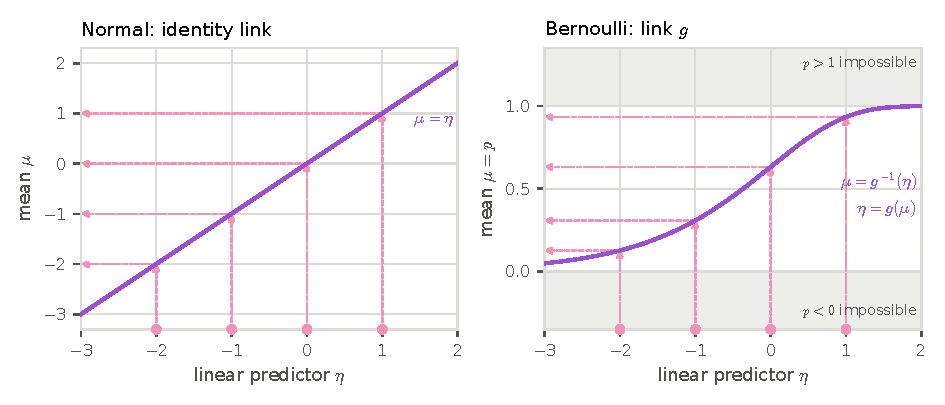
\includegraphics[width=\textwidth]{content/technical/figures/glm_link.pdf}
  \caption{The link function connects the mean $\mu$ of the outcome to the linear predictor $\eta$, shown for four equally spaced values of $\eta$ carried up to the curve and across to the mean. Left: in linear regression the link is the identity, so equal steps in $\eta$ give equal steps in $\mu$. Right: for a binary outcome the mean is the risk $p = g^{-1}(\eta)$, which stays between 0 and 1, so equal steps in $\eta$ give unequal steps in $p$.}
  \label{fig:tech-glm-link}
\end{figure}


\subsection{The Complementary Log-Log Link and the Hazard Ratio}
\label{sec:tech-segment-glmm}

One choice of $g$ is the complementary log-log (cloglog) link \cite[Section~7.3]{dobson2002glm}.
The link follows from an event that can occur at any time within the observation window but is observed only at its end.
% STUDY NOTE (2026-11-16, not printed).
%   Why cloglog, not logit: cloglog gives a hazard ratio that is the same over the whole window.
%   Logit gives an odds ratio, which changes with the baseline risk and the window length (Appendix B).
%   We never see when the event happened, only whether it had happened by the end. That is enough,
%   as long as the event cannot be undone (plaque does not disappear again).
Such an event is described through its hazard $h_i(t)$, which is the rate at which the event occurs at time $t$ among the units that are still event-free \cite[Section~10.2]{dobson2002glm}.
% STUDY NOTE (not printed).
%   The hazard acts only on the people who are still event-free, and that group shrinks.
%   Example: hazard 0.2 per year. Each year about 18% of those left get the event:
%   1000 -> 819 -> 670 ... The same percentage, but fewer people each year.
Integrated over the window $[0, \tau]$, the hazard gives the cumulative hazard $\Lambda_i$, and the probability of no event by the end of the window follows from it \cite[Section~10.2, Eq.~10.4]{dobson2002glm},
\begin{equation}
  \Lambda_i = \int_0^{\tau} h_i(t)\,dt ,
  \qquad
  1 - p_i = \exp(-\Lambda_i) .
  \label{eq:tech-cumhaz}
\end{equation}
% STUDY NOTE (not printed).
%   Lambda_i is the area under the hazard curve. It is NOT the linear predictor (that is log Lambda_i).
%   Why exp(-Lambda): staying event-free means getting through every small step of the window, so the
%   probabilities multiply. The log turns that product into a sum (the area), and exp turns it back.
%   Example: 0.99^10 = 0.904 = exp(-0.1005).
%   Why not 1 - Lambda: that would count people who already had the event again, and can go below 0.
%   The two are almost equal only when the event is rare.
%   We only learn the area, not the shape of the hazard curve over the window.
Under proportional hazards, the covariates multiply the hazard by the same factor throughout the window \cite[Section~10.2.2, Eq.~10.8]{dobson2002glm},
\begin{equation}
  h_i(t) = h_0(t) \exp\Bigl(\sum_k \beta_k x_{ik}\Bigr),
  \label{eq:tech-ph}
\end{equation}
where $h_0(t)$ is the hazard of a unit whose covariates are all zero, referred to as the baseline hazard.
% STUDY NOTE (not printed).
%   Baseline hazard = the shared curve. The covariates move each unit's curve up or down, so the
%   covariates are what make units differ. Hazard ratio 2 = twice as high at every time.
%   What the covariates miss goes into the frailty exp(b_i) (eq:tech-glmm) or is chance.
%   "All covariates zero" is an imaginary person unless the covariates are centred (then: an average person).
Integrating Eq.~\eqref{eq:tech-ph} over the window multiplies the cumulative hazard $\Lambda_0$ of this unit by the same factor, so the logarithm of the cumulative hazard is linear in the covariates \cite[Section~10.2.2]{dobson2002glm},
\begin{equation}
  \log\Lambda_i = \log\Lambda_0 + \sum_k \beta_k x_{ik} = \eta_i ,
  \label{eq:tech-logcumhaz}
\end{equation}
with the intercept of Eq.~\eqref{eq:tech-lp} equal to $\beta_0 = \log\Lambda_0$.
% STUDY NOTE (not printed).
%   Lambda_0 = area under the baseline hazard h_0(t).
%   beta_0 = log Lambda_0: the intercept is the log of the baseline area. Example: beta_0 = -2 gives
%   Lambda_0 = 0.135 and a baseline risk of 0.127.
%   A longer window gives a larger area, so beta_0 depends on the window; the hazard ratios do not.
%   Why log: Lambda cannot be negative, but a weighted sum can. The log fixes that.
%   Chain: hazard -> area Lambda -> log Lambda = linear predictor -> risk = 1 - exp(-Lambda).
Inserting $\Lambda_i = \exp(\eta_i)$ into Eq.~\eqref{eq:tech-cumhaz} gives the risk, and solving for $\eta_i$ gives the link itself,
\begin{equation}
  p_i = 1 - \exp\{-\exp(\eta_i)\},
  \qquad
  g(p_i) = \log\{-\log(1 - p_i)\} = \eta_i .
  \label{eq:tech-cloglog}
\end{equation}
The first expression is the inverse link $g^{-1}$ of Eq.~\eqref{eq:tech-link}.
The second takes the logarithm of minus the logarithm of the complement $1 - p_i$, which gives the link its name \cite[Section~7.3]{dobson2002glm}.

By Eq.~\eqref{eq:tech-ph}, an increase of one in $x_{ik}$ with the other covariates held fixed multiplies the hazard by $\exp(\beta_k)$ at every time in the window, referred to as the hazard ratio \cite[Section~10.2.2, Eq.~10.7]{dobson2002glm}.
The hazard ratio therefore compares two units that differ only in $x_{ik}$, and it is referred to as adjusted for the other covariates.
Its size depends on the scale on which $x_{ik}$ is measured, such as degrees or millimetres.
To compare covariates measured on different scales, each hazard ratio can be expressed per standard deviation of its covariate.

Units can differ in the time or the extent over which they are at risk, and this amount is their exposure $E_i$.
The exposure enters the linear predictor of Eq.~\eqref{eq:tech-logcumhaz} as $\gamma \log E_i$, so it multiplies the cumulative hazard by $E_i^{\gamma}$.
When $\gamma$ is fixed at 1, the cumulative hazard is proportional to the exposure and the term is referred to as an offset \cite[Section~9.2, Eq.~9.3]{dobson2002glm}.
When $\gamma$ is estimated instead, the data decide how strongly the cumulative hazard grows with the exposure.

\subsection{Clustered Outcomes and the Random Intercept}
\label{sec:tech-random-intercept}

The GLM treats all outcomes as independent \cite[Section~3.4]{dobson2002glm}.
This does not hold when units are grouped into clusters, such as several observations of the same person.
The units of a cluster share unmeasured traits, so their outcomes are correlated, and inference from a model that ignores the correlation is not valid \cite[Section~11.1]{dobson2002glm}.
A generalised linear mixed model (GLMM) accounts for the correlation by adding a random effect for each cluster to the linear predictor \cite[Section~11.5]{dobson2002glm}.
In its simplest form, the random effect is an intercept $b_i$ shared by all units of a cluster.
With $i$ now indexing the cluster and $j$ the unit within it, the risk of Eq.~\eqref{eq:tech-cloglog} becomes
\begin{equation}
  p_{ij}(b_i) = 1 - \exp\!\left\{-\exp(\eta_{ij} + b_i)\right\},
  \qquad
  b_i \sim \mathcal{N}(0, \sigma^2),
  \label{eq:tech-glmm}
\end{equation}
where $\eta_{ij}$ is the linear predictor of unit $j$ in cluster $i$ and $\sigma^2$ is the variance of the random intercepts.
The coefficients $\beta_k$ are the same for all clusters and are referred to as fixed effects, while $b_i$ differs between clusters, and a model with both is a mixed model.

Adding $b_i$ to the linear predictor multiplies the hazard of every unit in cluster $i$ by $\exp(b_i)$, referred to as the frailty of the cluster \cite[Section~2.2]{austin2017mhr}.
A cluster with a frailty above 1 is more prone to the event than its covariates suggest.
How much the frailty varies between clusters is summarised by the median hazard ratio (MHR) \cite[Section~2.2]{austin2017mhr}.
The MHR is the median ratio between the hazards of two units with the same covariates from two randomly chosen clusters, with the higher hazard divided by the lower.

The hazard ratio $\exp(\beta_k)$ in Eq.~\eqref{eq:tech-glmm} is conditional on $b_i$, so it compares units with the same frailty.
For a covariate that varies between the units of a cluster, this is a comparison within a cluster.
For a covariate that is the same for all units of a cluster, it is a comparison between two clusters with the same frailty.

\subsection{Likelihood Ratio Test and Cluster Risk}
\label{sec:tech-glmm-likelihood}

The parameters of the GLMM are estimated by maximum likelihood.
The random intercepts are not observed, so the likelihood is averaged over their distribution (Appendix~\ref{app:glmm-fitting}).
The joint contribution of a set of $q$ covariates is assessed with a likelihood ratio test.
The model is fitted with and without the set on the same units, and the two fits are compared through the statistic \cite[Sections~5.7 and~11.7]{dobson2002glm},
\begin{equation}
  \mathrm{LR} = 2\left(\ell_1 - \ell_0\right) \;\overset{H_0}{\sim}\; \chi^2_q ,
  \label{eq:tech-lr}
\end{equation}
where $\ell_1$ and $\ell_0$ denote the maximised log-likelihoods with and without the set.
Under the null hypothesis that the set adds no information, the statistic follows a $\chi^2$ distribution with $q$ degrees of freedom, and large values provide evidence against this hypothesis.
This reference distribution assumes that the random effects capture the dependence within clusters.
When some units of a cluster are more alike than others, a second random effect can be added for the subgroup (Appendix~\ref{app:glmm-variance}).

\label{sec:tech-aggregation}%
The fitted model also yields the risk that a cluster experiences the event in at least one of its units.
Let $A_i = 0$ denote that no unit of cluster $i$ has the event, and let $\Lambda_{ij} = \exp(\eta_{ij})$ denote the cumulative hazard of unit $j$ before the frailty is applied.
Assuming that the units of a cluster are independent given $b_i$, the probability of $A_i = 0$ is the product of the unit probabilities of no event.
Under the cloglog link, this product reduces to a sum, in which the cumulative hazards of the units add to a single cluster hazard,
\begin{equation}
  P(A_i = 0 \mid b_i) = \exp\!\left(-e^{b_i} H_i\right),
  \qquad
  H_i = \sum_{j=1}^{n_i} \Lambda_{ij} ,
  \label{eq:tech-agg-conditional}
\end{equation}
where $H_i$ is the summed cumulative hazard of the $n_i$ units.
For a new cluster the frailty is unknown, and the cluster risk is therefore obtained by averaging this probability over the distribution of $b_i$ (Appendix~\ref{app:glmm-risk}).
The cumulative hazard of a single unit is only one of the $n_i$ terms of $H_i$, so the association of a covariate with the event in that unit is diluted in the cluster hazard.
As a result, a set of covariates that is clearly associated with the event in Eq.~\eqref{eq:tech-lr} may change the cluster risk only slightly.
